\section{March 24}


\subsection{Segre class of a subscheme}

  \begin{definition}
    Let $X$ be a closed subscheme of a scheme $Y$. 
    The \emph{normal cone} of $X$ in $Y$ is defined as
    \[ C_{X/Y} \coloneqq \calSpec_X \bigoplus_{n\geq 0} \mathcal{I}^n/\mathcal{I}^{n+1}, \]
    where $\mathcal{I}$ is the ideal sheaf of $X$ in $Y$.
  \end{definition}

  If $Y$ is of pure dimension, then $C_{X/Y}$ is of pure dimension as well and $\dim C_{X/Y} = \dim Y$.

  \begin{example}
    When $X \injmap Y$ is a regular embedding, then $\calI$ is locally generated by a regular sequence of length $r$, $\calI/\calI^2$ is locally free of rank $r$, and $C_{X/Y} = N_{X/Y}$ is the normal bundle of $X$ in $Y$.

    When $X$ is a closed point $y \in Y$.
    Then $C_{X/Y}$ is the tangent cone of $Y$ at $y$.
    For instance, if $Y \subset \bbA^n$ is a hypersurface defined by a polynomial $f$ and $f_m$ is lowest degree homogeneous part of $f$, then $C_{0/Y}$ is the hypersurface defined by $f_m$ in $\bbA^n$.
    \[
      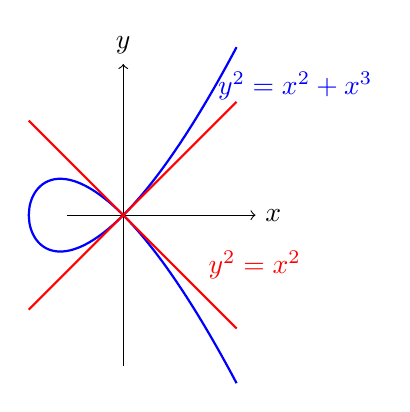
\begin{tikzpicture}[scale=1.2]
        \draw[->] (-0.6,0) -- (1.4,0) node[right] {$x$};
        \draw[->] (0,-1.6) -- (0,1.6) node[above] {$y$};

        \draw[blue, thick, domain=-1:1.2, samples=300, smooth]
          plot (\x, {\x*sqrt(\x + 1)});
        \draw[blue, thick, domain=-1:1.2, samples=300, smooth]
          plot (\x, {-\x*sqrt(\x + 1)});
        \node[blue, above right] at (0.9, 1.12) {$y^2=x^2+x^3$};

        \draw[red, thick, domain=-1:1.2, samples=300, smooth]
          plot (\x, \x);
        \draw[red, thick, domain=-1:1.2, samples=300, smooth]
          plot (\x, {-\x});
        \node[red, above right] at (0.8, -0.78) {$y^2=x^2$};
      \end{tikzpicture}
    \]
  \end{example}

  \begin{definition}
    For a closed subscheme $X \injmap Y$, the \emph{Segre class} of $X$ in $Y$ is defined as
    \[ s(X,Y) \coloneqq \sum_{k\geq 0} p_*(c_1(\calO(1))^k \cap [\bbP(C_{X/Y} \oplus \calO_X)]) \in \CH_*(X), \]
    where $p: \bbP(C_{X/Y} \oplus \calO_X) \to X$ is the projection.
  \end{definition}

  One can regard $\bbP(C_{X/Y} \oplus \calO_X)$ as the exceptional divisor $F$ of the blow-up of $Y \times \bbA^1$ along $X \times \{0\}$, 
  and $p$ as the restriction of the blow-up morphism to the exceptional divisor.
  Then 
  \[ s(X,Y) = \sum_{k\geq 0} (-1)^k \pi_*(F^{k+1}) \in \CH_*(X), \]
  where $\tilde{Y}$ is the blow-up of $Y \times \bbA^1$ along $X \times \{0\}$ and $F$ is the exceptional divisor.
  
  \begin{lemma}
    Let $Y$ be a pure-dimensional scheme of irreducible components $Y_1, \dots, Y_t$ with multiplicities $m_1, \dots, m_t$.
    Let $X$ be a closed subscheme of $Y$ and $X_u := X \cap Y_u$ for $u=1, \dots, t$.
    Then
    \[ s(X,Y) = \sum_{u=1}^t m_u s(X_u, Y_u). \]
  \end{lemma}
  \begin{proof}
    \Yang{}
  \end{proof}

  \begin{proposition}
    Let $f: Y' \to Y$ be a morphism of pure-dimensional schemes, $X \injmap Y$ a closed subscheme, and $g: X' := f^{-1}(X) \to X$ the preimage of $X$ in $Y'$.
    \begin{enumerate}
      \item If $f$ is proper, $Y$ is irreducible, $[Y'] = \sum_u m_u [Y'_u]$, and $f$ maps every irreducible component $Y'_u$ of $Y'$ onto $Y$, then
        \[ g_* s(X', Y') = \left(\sum_u m_u \deg(Y'_u/Y)\right) s(X,Y). \]
      \item If $f$ is flat of relative dimension $d$, then
        \[ g^* s(X,Y) = s(X', Y'). \]
    \end{enumerate}
  \end{proposition}
  \begin{proof}
    \Yang{}
  \end{proof}

  \begin{corollary}
    Let $Y$ be a variety, $X \injmap Y$ a closed subscheme, $E \injmap \tilde{Y} = \Bl_X Y$ the exceptional divisor, and $\eta: E \to X$ the projection.
    Then 
    \[ s(X,Y) = \eta_* \left( \sum_{k\geq 0} (-1)^k E^{k+1} \right). \]
  \end{corollary}
  \begin{proof}
    \Yang{}
  \end{proof}

  \begin{definition}\label{def:mult_of_variety_along_subvariety}
    Let $Y$ be a variety and $X \injmap Y$ a closed subvariety of codimension $r$.
    Define the \emph{multiplicity} of $Y$ along $X$ as
    \begin{align*}
        e_X Y &\coloneqq \text{ coefficient of } [X] \text{ in } s(X,Y) \in \CH_*(X) \\
        &= \text{ coefficient of } [X] \text{ in } (-1)^{r-1} \pi_*(E^{r}) \in \CH_*(X),
    \end{align*}
    where $\pi: \tilde{Y} = \Bl_X Y \to Y$ is the blow-up of $Y$ along $X$ and $E$ is the exceptional divisor.
  \end{definition}

  \begin{lemma}
    In the setting of \cref{def:mult_of_variety_along_subvariety}, we have 
    \[ e_X Y = \text{ the Samuel multiplicity of } Y \text{ along } X. \]
    That is, letting $A = \calO_{Y,X}$ be the local ring of $Y$ at the generic point of $X$ and $\frakm \subset A$ the maximal ideal, $\call_A(A/\frakm^{t+1}) = \dim_{\rkk(X)} \oplus_{i=0}^t \frakm^i/\frakm^{i+1}$ is a polynomial in $t$ for sufficiently large $t$, and the leading coefficient is $e_X Y / r!$.
  \end{lemma}
  \begin{proof}
    \Yang{}
  \end{proof}

  \begin{example}
    Let $Y$ be a variety, and $y \in Y$ be a closed point.
    Denote by $\pi: \tilde{Y} = \Bl_y Y \to Y$ the blow-up of $Y$ at $y$ and $E$ the exceptional divisor.
    If $y$ is a smooth point of $Y$, then $E \cong \bbP^{\dim Y - 1}$ and $e_y Y = 1$.
    If $y$ is an ordinary double point of $Y$, then $E$ is a smooth quadric hypersurface in $\bbP^{\dim Y}$ and $e_y Y = 2$.
  \end{example}


\subsection{Intersection products and Gysin maps}

  Let $f: X \injmap Y$ be a regular embedding of codimension $r$.

  \textbf{Goal:} for all subvariety $V \subset Y$ of dimension $i$, define $X \cdot V \in \CH_{i-r}(X)$ and the Cysin map $f^*: \CH_i(Y) \to \CH_{i-r}(X),\ [V] \mapsto X \cdot V$. 
  Even when $V$ is not properly intersecting with $X$, these should be well-defined.

  We have defined some special Gysin maps:
  \begin{itemize}
    \item let $X$ be a scheme and $f: D \injmap X$ a Cartier divisor, 
      then $f^*: \CH_i(X) \to \CH_{i-1}(D)$ is defined by $\alpha \mapsto D \cdot \alpha$;
    \item let $\pi: E \to X$ be a vector bundle of rank $r$ and $s: X \to E$ the zero section, 
      recall $\pi^*: \CH_i(X) \isomap \CH_{i+r}(E)$, 
      and define $s^* = (\pi^*)^{-1}: \CH_{i+r}(E) \isomap \CH_i(X)$.
  \end{itemize}

  Consider the cell decomposition diagram:
  \[
    \begin{tikzcd}
      \bbP(E) \ar[r, hook, "f"] \ar[dr, "p"'] & \bbP(E \oplus \calO_X) \ar[d, "q"] & E \ar[l, hook', "g"'] \ar[ld, "\pi"] \\
         & X, &
    \end{tikzcd}
  \]
  we have the Euler sequence
  \[ 0 \to \calO(-1) \to q^*(E \oplus \calO_X) \to T_{\bbP(E \oplus \calO_X)/X}(-1) \to 0. \]

  \begin{proposition}
    In the above setting, let $\beta \in \CH_i(E)$ and $\overline{\beta} \in \CH_i(\bbP(E \oplus \calO_X))$ such that $g^* \overline{\beta} = \beta$.
    Then $s^* \beta = q_* (c_1(\calO(1))^r \cap \overline{\beta})$.
  \end{proposition}
  \begin{proof}
    \Yang{}
  \end{proof}

  \begin{example}
    Let $\pi: E \to X$ be a vector bundle of rank $r$ on a scheme $X$ and $s: X \to E$ the zero section.
    Then $s^* s_* \alpha = c_r(E) \cap \alpha$ for all $\alpha \in \CH_*(X)$.

    Indeed, for $\beta = s_* \alpha$, 

    \Yang{}
  \end{example}

  \begin{construction}[Intersection product]\label{constr:intersection_product_for_regular_embedding}
    Let $f: X \injmap Y$ be a regular embedding of codimension $r$ and $V \subset Y$ a subvariety of dimension $i$.
    Consider the fiber product diagram
    \[
      \begin{tikzcd}
        W \ar[r, "f'"] \ar[d, "g'"'] & V \ar[d, hook, "g"] \\
        X \ar[r, hook, "f"] & Y.
      \end{tikzcd}
    \] 
    Then $\calI_X \cdot \calO_V = \calI_W$ and 
    \[ \left( \bigoplus_{n\geq 0} \calI_X^n/\calI_X^{n+1} \right) \otimes_{\calO_X} \calO_W \surjmap \bigoplus_{n\geq 0} \calI_W^n/\calI_W^{n+1}, \]
    which induces a closed embedding $C_{W/V} \injmap g^* N_{X/Y} \eqqcolon N$.
    Let $s: W \to N$ be the zero section, define 
    \[ X \cdot V \coloneqq s^* [C_{W/V}] \in \CH_{i-r}(X). \]
  \end{construction}

  \begin{proposition}
    In the above setting, we have the following properties.
    \begin{enumerate}
      \item $X \cdot V = \Big( c(N) \cap s(W,V) \Big)_{i-r} \in \CH_{i-r}(X)$, where the subscript $i-r$ means taking the component of dimension $i-r$;
      \item $X \cdot V = q_* \left( c_r(\xi) \cap [\bbP(C_{W/V} \oplus \calO_W)] \right) \in \CH_{i-r}(X)$, where $q: \bbP(C_{W/V} \oplus \calO_W) \to W$ is the projection and $\xi$ is the universal quotient bundle on $\bbP(C_{W/V} \oplus \calO_W)$;
      \item when $r=1$, (i.e. $X$ is a Cartier divisor) and $f$ is a closed embedding, $X \cdot V$ agrees with the previous definition of intersection product for Cartier divisors.
    \end{enumerate}
  \end{proposition}
  \begin{proof}
    \Yang{}
  \end{proof}